\documentclass{beamer}

\usepackage{Haust2016glærur}

\title{Stærðfræðimynstur í tölvunarfræði}
\subtitle{Vika 10, seinni fyrirlestur}

\begin{document}

\begin{frame}
\titlepage
\end{frame}


\section{Inngangur}

\begin{frame}{Í síðasta tíma}
\begin{itemize}
 \item Net
 \item Hagnýting neta
 \item Nokkur hugtök sem tengjast netum
\end{itemize}
\end{frame}

\section{Eiginleikar neta}

\begin{frame}{Handabandssetningin}
Upprifjun:
\begin{tcolorbox}[title=Handabandssetningin]
Látum $G = (V, E)$ vera óstefnt net með $m$ leggjum. Þá er
\[
 2m = \sum_{v \in V} \deg(v)
\]
\end{tcolorbox}
Handabandssetningin (e. \emph{the handshake theorem}) á við um fjölnet og net með lykkjum.
\end{frame}

\begin{frame}{Hnútar af oddatölustigi}
\begin{tcolorbox}
Fjöldi hnúta af oddatölustigi í óstefndu neti er slétt tala.
\end{tcolorbox}

Stutt sönnun: Látum $G = (V,E)$ vera óstefnt net. Látum $V_s$ vera mengi hnúta $G$ sem eru af stigi með slétta tölu og $V_o$ vera mengi hnúta $G$ sem eru af oddatölustigi. Nú er
\[
 2m = \sum_{v \in V} \deg(v) = \sum_{v \in V_s} \deg(v) + \sum_{v \in V_o} \deg(v).
\]
Þar sem $2m$ er slétt tala og $\sum_{v \in V_s} \deg(v)$ er slétt tala hlýtur $\sum_{v \in V_o} \deg(v)$ að vera slétt tala. Summa af oddatölum er einungis slétt þegar fjöldi oddatalnanna er sléttur, svo fjöldi oddatöluhnúta er sléttur.
\end{frame}

\begin{frame}{Stefnd net og stig}
\begin{itemize}
 \item Í stefndu neti getum við skilgreint: innstig (e. \emph{in-degree}) og útstig (e. \emph{out-degree}) hnúta
 \begin{itemize}
  \item Innstig hnúts $v$ er táknað með $\deg^-(v)$ og er fjöldi örvaleggja sem hefur $v$ sem lokahnút
  \item Útstig hnúts $v$ er táknað með $\deg^+(v)$ og er fjöldi örvaleggja sem hefur $v$ sem upphafshnút
 \end{itemize}
\end{itemize}
\end{frame}

\begin{frame}{Dæmi}
\begin{columns}
\column{0.6\textwidth}
Hver eru innstig og útstig hnútanna í netinu hér að neðan?

\vspace{0.5cm}
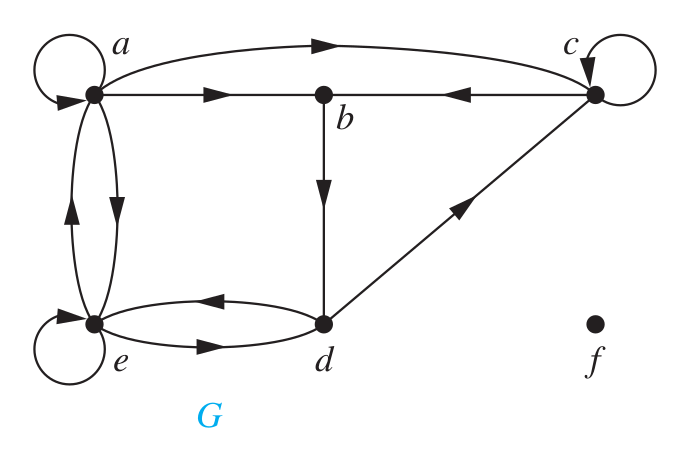
\includegraphics[width=\linewidth]{indegree-outdegree}
\pause
\column{0.4\textwidth}
\begin{tabular}{ccc}
\toprule
Hnútur&Innstig&Útstig\\
\midrule
$a$&2&4\\
$b$&2&1\\
$c$&3&2\\
$d$&2&2\\
$e$&3&3\\
$f$&0&0\\
\bottomrule
\end{tabular}
\end{columns}
\end{frame}

\begin{frame}{Innstig og útstig}
Hver stefndur leggur/örvaleggur er með upphafshnút og lokahnút, svo við getum sett fram staðhæfingu:

\begin{tcolorbox}
Látum $G = (V,E)$ vera stefnt net. Þá er
\[
\sum_{v\in V} \deg^-(v) = \sum_{v\in V} \deg^+(v) = |E|
\]
\end{tcolorbox}

\end{frame}

\section{Sérstök net}

\begin{frame}{Sérstök net}
\begin{itemize}
 \item Ýmis net hafa sérstakar uppbyggingar
 \item Nefnum sérstaklega:
 \begin{itemize}
  \item Tóm net (e. \emph{empty graph})
  \item Núllnet (e. \emph{null graph})
  \item Fullskipuð net (e. \emph{complete graph})
  \item Hringa (e. \emph{cycles})
  \item Hjól (e. \emph{wheels}
  \item $n$-tengingar (e. \emph{$n$-cubes})
 \end{itemize}
\end{itemize}
\end{frame}

\begin{frame}{Tóm net og núllnet}
\begin{tcolorbox}[title=Tómt net]
Tómt net er net $G = (V, E)$ þar sem $E = V = \emptyset$. Þ.e.a.s. net er tómt ef það inniheldur enga leggi og enga hnúta.
\end{tcolorbox}

\begin{tcolorbox}[title=Núllnet]
Núllnet er net $G = (V, E)$ þar sem $E = \emptyset$. Þ.e.a.s. net er núllnet ef það inniheldur enga leggi til að tengja hnúta þess saman.
\end{tcolorbox}
Ath: Nöfnunum á þessum skilgreiningum er stundum víxlað!
\end{frame}

\begin{frame}{Fullskipuð net}
\begin{tcolorbox}[title=Fullskipað net]
Fullskipað net með $n$ hnútum er einfalt net sem hefur nákvæmlega einn legg á milli hverra tveggja aðskildra hnúta. Fullskipað net með $n$ hnútum er táknað með $K_n$.
\end{tcolorbox}

\begin{center}
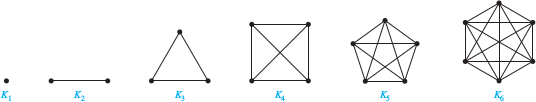
\includegraphics[width=\linewidth]{graph-complete}
\end{center}

\end{frame}

\begin{frame}{Hringur}
\begin{tcolorbox}[title=Hringur]
Hringur með $n \geq 3$ hnútum er einfalt net með hnúta $v_1, v_2, \ldots, v_n$ og leggi $\{v_1 , v_2\},
\{v_2 , v_3 \}, \ldots , \{v_{n-1} , v_n \}$, og $\{v_n , v_1 \}$. Hringur með $n$ hnútum er táknaður með $C_n$.
\end{tcolorbox}

\begin{center}
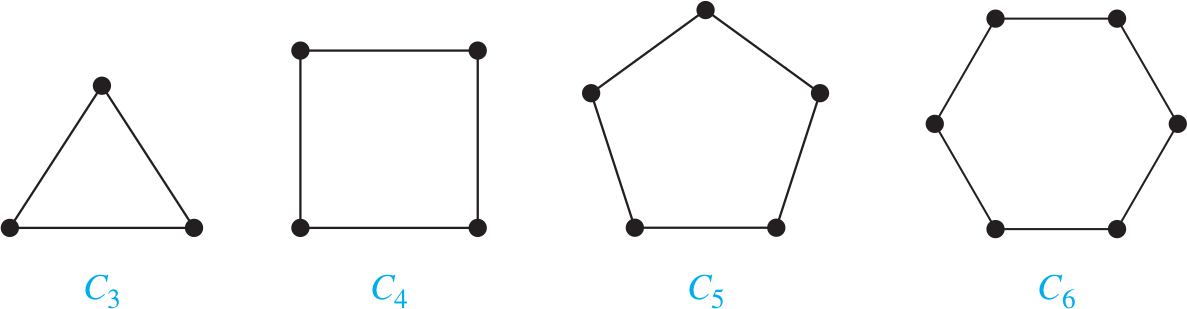
\includegraphics[width=\linewidth]{graph-cycle}
\end{center}

\end{frame}

\begin{frame}{Hjól}
\begin{tcolorbox}[title=Hjól]
Hjólið $W_n$ er myndað með því að taka hringinn $C_n$ og bæta við það einum hnúti og leggjum sem tengja nýja hnútinn við sérhvern hnút í $C_n$. Hjólið $W_n$ er þá með $n+1$ hnút.
\end{tcolorbox}

\begin{center}
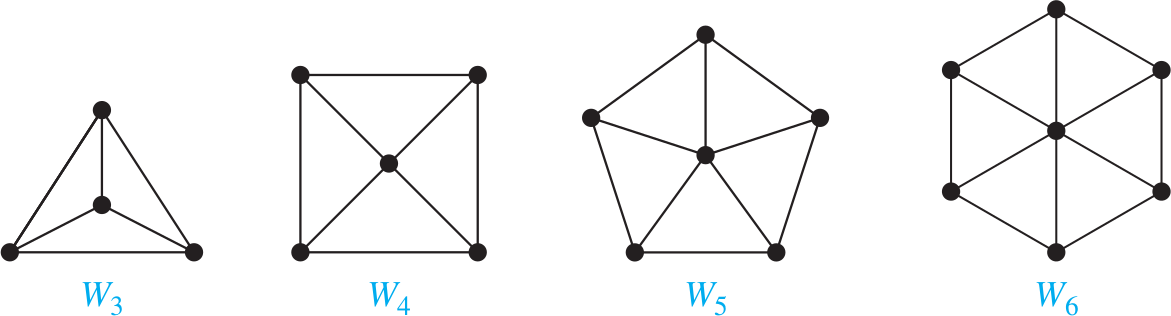
\includegraphics[width=\linewidth]{graph-wheel}
\end{center}
\end{frame}

\begin{frame}{$n$-teningur}
\begin{tcolorbox}[title=$n$-teningur]
$n$-tengingur, eða ``$n$-víður ofurteningur'' er táknaður með $Q_n$.

Látum $Q_0$ vera netið sem samanstendur af einum hnút og engum leggjum. Þá má búa til $Q_{n+1}$ út frá $Q_n$ með því að taka alla hnúta í $Q_n$, afrita þá, og bæta legg við á milli hvers upphaflegs hnúts og afrits hans.
\end{tcolorbox}

\begin{center}
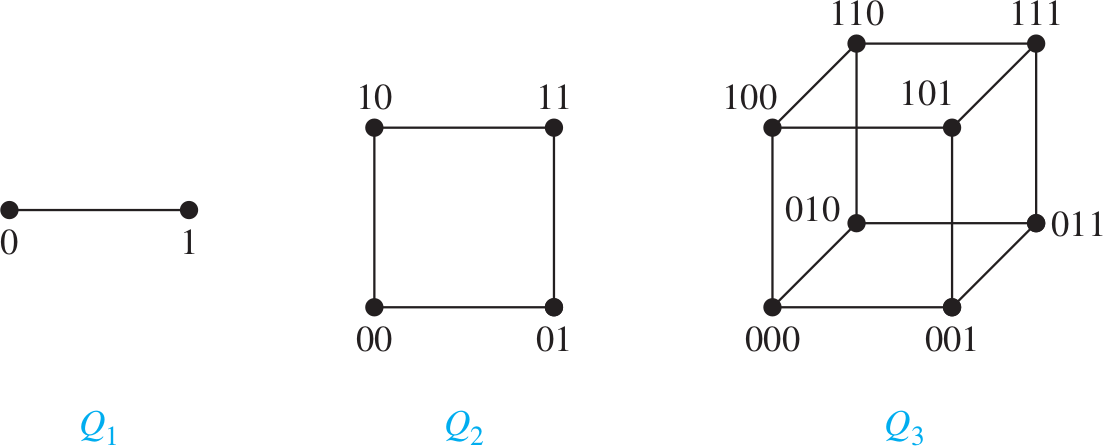
\includegraphics[width=\linewidth]{graph-n-cube}
\end{center}
\end{frame}

\section{Tvíhlutanet}

\begin{frame}{Tvíhlutanet}
Net sem kallast tvíhlutanet hafa eiginleika sem vert er að skoða sérstaklega.
\begin{tcolorbox}[title=Tvíhlutanet]
Einfalt net $G = (V,E)$ kallast tvíhlutanet (e. \emph{bipartite graph}) megi skipta $V$ í tvö aðskilin mengi $V_1$ og $V_2$ þannig að allir leggir í netinu hafa annan endapunkt sinn í $V_1$ og hinn í $V_2$. Þá mynda mengin $V_1$ og $V_2$ tvískiptingu (e. \emph{bipartition}) á hnútamengi $G$.
\end{tcolorbox}

\end{frame}

\begin{frame}{Dæmi}
Er hringurinn $C_6$ tvíhlutanet? \pause

\begin{center}
Já!

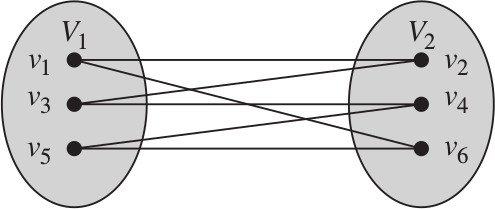
\includegraphics[width=0.8\textwidth]{graph-bipartite-c6}
\end{center}
\end{frame}

\begin{frame}{Litun á tvíhlutaneti}
Við getum inleitt hugmyndina um litun á neti (e. \emph{graph coloring}) til að auðvelda okkur að kanna hvort að net sé tvíhlutanet eða ekki.

\begin{tcolorbox}[title=Litun tvíhlutanets]
Einfalt net er tvíhlutanet þá og því aðeins að hægt sé að lita hvern hnút netsins með einum af tveimur litum á þann hátt að enginn hnútur fái sama lit og nágranni sinn.
\end{tcolorbox}

\end{frame}

\begin{frame}{Dæmi}
Eru netin $G$ og $H$ tvíhlutanet?

\begin{center}
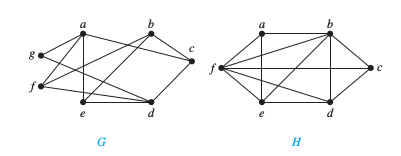
\includegraphics[width=0.8\textwidth]{graph-bipartite-coloring}
\end{center}
\pause

$G$ er tvíhlutanet, $H$ ekki.
\end{frame}

\begin{frame}{Fullskipuð tvíhlutanet}
Fullskipað tvíhlutanet $K_{m, n}$ er net sem mynda má á tvíhlutaskiptingu $\{V_1, V_2\}$ þar sem $|V_1| =m, |V_2|=n$ og með legg á milli tveggja hnúta þá og því aðeins að annar endahnútur leggsins sé í $V_1$ og hinn í $V_2$.
\end{frame}

\section{Spyrðingar}

\begin{frame}{Spyrðingar}
\begin{tcolorbox}[title=Spyrðing]
Spyrðing (e. \emph{matching}) í einföldu neti $G = (V, E)$ er hlutmengi $E$ sem hefur þann eiginleika að engir tveir leggir eigi sameiginlegan endahnút.
\end{tcolorbox}
Önnur leið til að sjá fyrir sér spyrðingu: Séu leggirnir $\{s, t\}$ og $\{u, v\}$ aðskildir leggir í spyrðingu, þá eru hnútarnir $s, t, u$ og $v$ aðskildir hnútar.
\end{frame}

\begin{frame}{Dæmi}
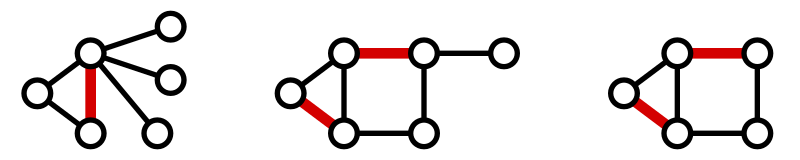
\includegraphics[width=\textwidth]{matching-maximal}
\end{frame}

\begin{frame}{Eiginleikar spyrðinga}
\begin{itemize}
 \item Spyrðing í neti er af hámarksstærð (e. \emph{maximum matching}) ef ekki er til spyrðing sem tekur til fleiri leggja í netinu
 \item Spyrðing í neti er fullkomin (e. \emph{complete}) ef sérhver hnútur í netinu er endi einhvers leggs hennar
 \begin{itemize}
  \item Bókin skilgreinir sérstaklega ákveðna gerð fullkominnar spyrðingar fyrir tvíhlutanet
  \item Spyrðing $M$ í tvíhlutanetinu $G=(V, E)$ með tvíhlutaskiptingu $\{V_1, V_2\}$ er fullkomin frá $V_1$ til $V_2$ sé sérhver hnútur í $V_1$ endahnútur einhvers leggs í spyrðingunni 
 \end{itemize}
\end{itemize}
\end{frame}

\begin{frame}{Dæmi}
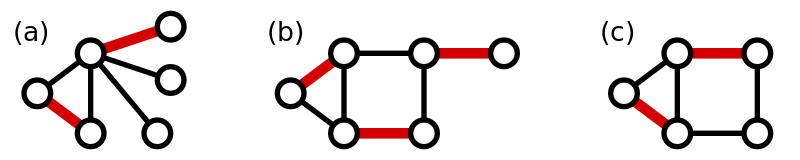
\includegraphics[width=\textwidth]{matching-maximum}
\end{frame}

\begin{frame}{Setning Hall's}
Getum sett fram setningu um tilvist fullkominnar spyrðingar milli hluta tvíhlutanets.

\begin{tcolorbox}[title=Setning Halls]
Tvíhlutanetið $G = (V, E)$ með tvíhlutaskiptinguna $\{V_1, V_2\}$ hefur fullkomna spyrðingu frá $V_1$ til $V_2$ ef og aðeins ef $|N(A)| \geq |A|$ fyrir öll hlutmengi $A$ í $V_1$.
\end{tcolorbox}

Þessi setning er stundum kölluð ``Giftingarsetning'' Halls.
\end{frame}

\section{Framsetning á netum}

\begin{frame}{Framsetning á netum}
\begin{itemize}
 \item Það að teikna net upp er ekki alltaf vænlegur kostur
 \item Skoðum þrjá möguleika sem við höfum til að setja net fram
 \begin{itemize}
  \item Grennslalistar (e. \emph{adjacency lists})
  \item Grennslafylki (e. \emph{adjacency matrices})
  \item Legufylki (e. \emph{incidence matrices})
 \end{itemize}
\end{itemize}
\end{frame}

\begin{frame}{Grennslalistar}
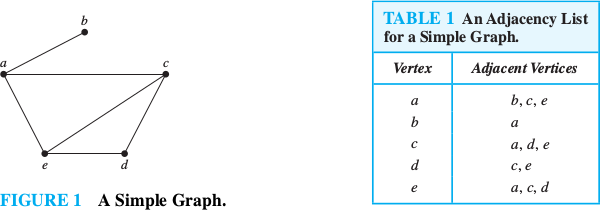
\includegraphics[width=\textwidth]{adjacency-lists}
\end{frame}

\begin{frame}{Grennslafylki}
Látum $G = (V, E)$ vera einfalt net með $|V| = n$ og búum til röðun á hnútunum $v_1, v_2, \ldots v_n$. Legufylkið $A_G$ m.t.t. þessarar röðunar er þá $n \times n$ fylki $[a_{ij}]$ þar sem $a_{ij}$ er 1 sé $\{v_i,v_j\}$ leggur í fylkinu og 0 annars.

Dæmi, með hnútaröðunina í stafrófsröð:
\begin{center}
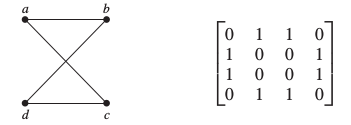
\includegraphics[width=0.6\textwidth]{adjacency-matrix}
\end{center}
Væri netið ekki einfalt gætum við sett hærri tölur í sætin. Grennslafylki fyrir stefnt net væri ekki endilega samhverft.
\end{frame}

\begin{frame}{Legufylki}
Látum $G = (V, E)$ vera óstefnt net með $V = \{v_1, v_2, \ldots, v_n\}$ og $E = \{e_1, e_2, \ldots, e_m\}$. Legufylki netsins m.t.t. þessara raðana er þá $n \times m$ fylki $[m_{ij}]$ þar sem $m_{ij}$ er 1 sé leggurinn $e_j$ tengdur hnútnum $v_i$, annars 0.

Dæmi:
\begin{center}
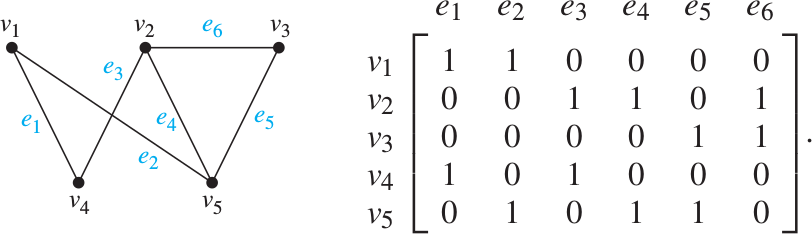
\includegraphics[width=0.6\textwidth]{incidence-matrix}
\end{center}
Lykkja myndar dálk með einum ás. Í fjölneti eru endurteknir dálkar.
\end{frame}


\begin{frame}{Að skrifa net í forritunarmáli}
\begin{itemize}
 \item Til að framkvæma útreikninga með gögnum sem tengjast netum þarf að koma netinu inn í tölvuna
 \item Mismunandi leiðir viðeigandi eftir forritunarmálum
 \begin{itemize}
  \item Java: Klasi? (Líklega grennslalistar)
  \item Matlab: Fylki? 
  \item Python: Dictionaries? (Líklega grennslalistar)
  \item C++: Structure? (Líklega grennslalistar)
 \end{itemize}
\end{itemize}
\end{frame}

\begin{frame}{Næst}
Samhengi neta (10.3), kannski Euler- og Hamilton vegir (10.4).
\end{frame}


\end{document}
